% Options for packages loaded elsewhere
\PassOptionsToPackage{unicode}{hyperref}
\PassOptionsToPackage{hyphens}{url}
\documentclass[
  11pt,
  a4paper,
]{article}
\usepackage{xcolor}
\usepackage[top=2.0cm,bottom=2.0cm,left=2.0cm,right=2.0cm]{geometry}
\usepackage{amsmath,amssymb}
\setcounter{secnumdepth}{-\maxdimen} % remove section numbering
\usepackage{iftex}
\ifPDFTeX
  \usepackage[T1]{fontenc}
  \usepackage[utf8]{inputenc}
  \usepackage{textcomp} % provide euro and other symbols
\else % if luatex or xetex
  \usepackage{unicode-math} % this also loads fontspec
  \defaultfontfeatures{Scale=MatchLowercase}
  \defaultfontfeatures[\rmfamily]{Ligatures=TeX,Scale=1}
\fi
\usepackage{lmodern}
\ifPDFTeX\else
  % xetex/luatex font selection
  \setmainfont[]{Times New Roman}
  \setsansfont[]{Arial}
  \setmonofont[]{Menlo}
\fi
% Use upquote if available, for straight quotes in verbatim environments
\IfFileExists{upquote.sty}{\usepackage{upquote}}{}
\IfFileExists{microtype.sty}{% use microtype if available
  \usepackage[]{microtype}
  \UseMicrotypeSet[protrusion]{basicmath} % disable protrusion for tt fonts
}{}
\makeatletter
\@ifundefined{KOMAClassName}{% if non-KOMA class
  \IfFileExists{parskip.sty}{%
    \usepackage{parskip}
  }{% else
    \setlength{\parindent}{0pt}
    \setlength{\parskip}{6pt plus 2pt minus 1pt}}
}{% if KOMA class
  \KOMAoptions{parskip=half}}
\makeatother
\usepackage{longtable,booktabs,array}
\newcounter{none} % for unnumbered tables
\usepackage{calc} % for calculating minipage widths
% Correct order of tables after \paragraph or \subparagraph
\usepackage{etoolbox}
\makeatletter
\patchcmd\longtable{\par}{\if@noskipsec\mbox{}\fi\par}{}{}
\makeatother
% Allow footnotes in longtable head/foot
\IfFileExists{footnotehyper.sty}{\usepackage{footnotehyper}}{\usepackage{footnote}}
\makesavenoteenv{longtable}
\setlength{\emergencystretch}{3em} % prevent overfull lines
\providecommand{\tightlist}{%
  \setlength{\itemsep}{0pt}\setlength{\parskip}{0pt}}
% 1-column header for CystoDS section report
\PassOptionsToPackage{table,xcdraw}{xcolor}
\usepackage[section]{placeins}
\usepackage{caption}
\usepackage{fancyhdr}
\usepackage{titlesec}
\usepackage{enumitem}
\usepackage{seqsplit}
\usepackage{booktabs}
\usepackage{graphicx}
\usepackage{microtype}
\usepackage{tabularx}
\usepackage{adjustbox}
\usepackage{float}

\definecolor{CystoBlue}{HTML}{1F4E79}
\definecolor{CystoTeal}{HTML}{2A7F62}
\definecolor{CystoGray}{HTML}{4A5568}
\definecolor{CystoDark}{HTML}{1A202C}

\graphicspath{{../../Docs/}{Docs/}{paper_assets/}{../paper_assets/}}

\captionsetup{font=small,labelfont={bf,color=CystoBlue}}
\captionsetup[table]{position=top,skip=3pt}
\captionsetup[figure]{position=bottom,skip=4pt}

\renewcommand{\figurename}{Hình}
\renewcommand{\tablename}{Bảng}

\titleformat{\section}{\Large\bfseries\color{CystoBlue}}{\thesection.}{0.4em}{}
\titleformat{\subsection}{\large\bfseries\color{CystoTeal}}{\thesubsection.}{0.4em}{}
\titleformat{\subsubsection}{\normalsize\bfseries\color{CystoDark}}{\thesubsubsection.}{0.4em}{}

\setlength{\parindent}{1.0em}
\setlength{\parskip}{0.35em plus 0.05em minus 0.05em}
\setlist{nosep,leftmargin=1.5em,topsep=0.3em}

\pagestyle{fancy}
\fancyhf{}
\fancyhead[L]{\small\color{CystoGray}CystoDS -- Báo Cáo Trực Quan Hóa Grad-CAM \& Định Vị Không Gian}
\fancyhead[R]{\small\color{CystoGray}CystoDS 2026}
\fancyfoot[C]{\small\color{CystoGray}\thepage}
\setlength{\headheight}{14pt}
\renewcommand{\headrulewidth}{0.35pt}

\AtBeginDocument{%
  \hypersetup{
    colorlinks=true,
    linkcolor=CystoBlue,
    urlcolor=CystoTeal,
    citecolor=CystoBlue,
  }%
}
\usepackage{bookmark}
\IfFileExists{xurl.sty}{\usepackage{xurl}}{} % add URL line breaks if available
\urlstyle{same}
\hypersetup{
  pdftitle={CystoDS: Báo Cáo Trực Quan Hóa Grad-CAM \& Đánh Giá Định Vị Không Gian},
  hidelinks,
  pdfcreator={LaTeX via pandoc}}

\title{CystoDS: Báo Cáo Trực Quan Hóa Grad-CAM \& Đánh Giá Định Vị Không
Gian}
\usepackage{etoolbox}
\makeatletter
\providecommand{\subtitle}[1]{% add subtitle to \maketitle
  \apptocmd{\@title}{\par {\large #1 \par}}{}{}
}
\makeatother
\subtitle{Đánh giá định tính và định lượng độ trùng khớp Grad-CAM IoU
giữa Swin Baseline và Mô Hình Đề Xuất 3S-HFT v3.1 trên Ground-Truth
Mask}
\author{}
\date{Báo cáo nghiên cứu 2026}

\begin{document}
\maketitle

\section{CystoDS: Báo Cáo Trực Quan Hóa Grad-CAM \& Đánh Giá Định Vị
Không
Gian}\label{cystods-buxe1o-cuxe1o-trux1ef1c-quan-huxf3a-grad-cam-ux111uxe1nh-giuxe1-ux111ux1ecbnh-vux1ecb-khuxf4ng-gian}

\subsection{Đánh giá định tính và định lượng độ trùng khớp Grad-CAM IoU
giữa Swin Baseline và Mô Hình Đề Xuất 3S-HFT v3.1 trên Ground-Truth
Mask}\label{ux111uxe1nh-giuxe1-ux111ux1ecbnh-tuxednh-vuxe0-ux111ux1ecbnh-lux1b0ux1ee3ng-ux111ux1ed9-truxf9ng-khux1edbp-grad-cam-iou-giux1eefa-swin-baseline-vuxe0-muxf4-huxecnh-ux111ux1ec1-xuux1ea5t-3s-hft-v3.1-truxean-ground-truth-mask}

\section{CystoDS: Báo Cáo Trực Quan Hóa Grad-CAM \& Đánh Giá Định Vị
Không Gian (Explainability \& Localization
Analysis)}\label{cystods-buxe1o-cuxe1o-trux1ef1c-quan-huxf3a-grad-cam-ux111uxe1nh-giuxe1-ux111ux1ecbnh-vux1ecb-khuxf4ng-gian-explainability-localization-analysis}

\subsection{1. Mục Tiêu \& Bối Cảnh Nghiên
Cứu}\label{mux1ee5c-tiuxeau-bux1ed1i-cux1ea3nh-nghiuxean-cux1ee9u}

Bên cạnh các chỉ số phân loại thống kê (AUROC, Accuracy, Macro-F1), việc
chứng minh tính minh bạch và độ tin cậy không gian của mô hình học sâu
trong chẩn đoán hình ảnh y tế đóng vai trò then chốt cho sự chấp thuận
của các phẫu thuật viên niệu khoa. Trong phẫu thuật nội soi bàng quang,
một mô hình đạt độ chính xác phân loại cao nhưng lại đưa ra quyết định
dựa trên các điểm ảnh nền (background artifacts), phản xạ ánh sáng
(specular glare) hay viền đen của camera sẽ tiềm ẩn nguy cơ chẩn đoán
sai lầm nghiêm trọng trên lâm sàng.

Nghiên cứu này triển khai phân tích định vị không gian và khả năng giải
thích được (\textbf{Explainability \& Localization Analysis}) thông qua
kỹ thuật \textbf{Grad-CAM (Gradient-weighted Class Activation Mapping)},
nhằm trả lời hai câu hỏi cốt lõi: 1. \emph{Mô hình đề xuất
\textbf{Proposed 3S-HFT v3.1} có tập trung vào đúng vùng tổn thương bệnh
học mà bác sĩ chuyên khoa đã khoanh vùng (\textbf{Ground-Truth Detection
Mask}) tốt hơn mô hình \textbf{Swin Baseline (Single-Task Fine-Level
Classifier)} hay không?} 2. \emph{Sự vượt trội về mặt định tính
(Qualitative Heatmaps) có được củng cố bằng bằng chứng định lượng nhất
quán (\textbf{Grad-CAM Intersection over Union - IoU}) trên các nhóm
bệnh lý khác nhau hay không?}

\begin{center}\rule{0.5\linewidth}{0.5pt}\end{center}

\subsection{2. Giao Thức Thực Nghiệm Chuẩn Hóa (Final Experimental
Protocol)}\label{giao-thux1ee9c-thux1ef1c-nghiux1ec7m-chuux1ea9n-huxf3a-final-experimental-protocol}

Nhằm đảm bảo tính khách quan và loại bỏ hoàn toàn thiên lệch lựa chọn
mẫu (\emph{selection bias}), giao thức Grad-CAM được thiết lập nghiêm
ngặt:

\begin{enumerate}
\def\labelenumi{\arabic{enumi}.}
\tightlist
\item
  \textbf{Mô hình đối chuẩn:}

  \begin{itemize}
  \tightlist
  \item
    \textbf{Swin Baseline:} Mô hình Swin-Tiny huấn luyện đơn nhiệm ở
    tầng vi thể (\emph{Single-Task Fine-Level Classifier}), lấy trực
    tiếp từ điểm kiểm tra (\emph{checkpoint}) tốt nhất của \textbf{Split
    0} trên Hugging Face.
  \item
    \textbf{Proposed Model (3S-HFT v3.1):} Mô hình Swin-Tiny huấn luyện
    đa tầng tuần tự kết hợp \emph{Curriculum Warmup} và \emph{Smoothed
    Balanced Softmax}, lấy từ checkpoint tốt nhất của \textbf{Split 0}.
  \end{itemize}
\item
  \textbf{Đối tượng phân tích (5 Phân Lớp Vi Thể Đại Diện):}

  \begin{itemize}
  \tightlist
  \item
    Đánh giá trực tiếp trên \textbf{Fine-level class prediction} (cùng
    chung target logit vi thể giữa 2 mô hình).
  \item
    Tuyển chọn 5 phân lớp đại diện cho 3 nhóm Coarse lớn trong hệ thống
    phân loại:

    \begin{itemize}
    \tightlist
    \item
      \textbf{Malignant (Ác tính):} \emph{LowGradePapillary} (U nhú độ
      thấp) và \emph{HighGradePapillary} (U nhú độ cao).
    \item
      \textbf{Foreign bodies (Dị vật / Ngoại lai):} \emph{AirBubble}
      (Bọt khí nội soi).
    \item
      \textbf{Anatomical landmarks (Mốc giải phẫu):}
      \emph{UreteralOrifice} (Lỗ niệu quản) và \emph{ResectionScar} (Sẹo
      cắt đốt TURBT).
    \end{itemize}
  \end{itemize}
\item
  \textbf{Tiêu chuẩn chọn mẫu True-Positive (TP):}

  \begin{itemize}
  \tightlist
  \item
    Mỗi phân lớp chọn \textbf{1 mẫu True-Positive (TP)} đại diện
    (\(\text{Ground Truth} = \text{Prediction}_{\text{Baseline}} = \text{Prediction}_{\text{Proposed}} = \text{Fine Class}\)).
  \item
    Các mẫu thuộc các lớp tổn thương phổ biến được trích xuất hoàn toàn
    từ \textbf{tập Test độc lập 100\% bệnh nhân của Split 0}.
  \end{itemize}
\item
  \textbf{Trích xuất đặc trưng \& Công thức tính Grad-CAM:}

  \begin{itemize}
  \tightlist
  \item
    Cả hai mô hình đều trích xuất bản đồ kích hoạt không gian và
    gradient tại tầng chuẩn hóa cuối cùng của Stage 4
    (\texttt{encoder.layers{[}-1{]}.blocks{[}-1{]}.norm1}, kích thước
    không gian \(7 \times 7 \times 768\)).
  \item
    Bản đồ nhiệt CAM được nội suy song tuyến (\emph{bilinear
    interpolation}) về kích thước \(224 \times 224\) và chuẩn hóa cường
    độ về đoạn \([0, 1]\):
    \[CAM_{\text{norm}}(x, y) = \frac{CAM(x,y) - \min(CAM)}{\max(CAM) - \min(CAM)}\]
  \end{itemize}
\item
  \textbf{Chỉ số định lượng Grad-CAM IoU:}

  \begin{itemize}
  \tightlist
  \item
    Áp dụng ngưỡng nhị phân hóa cố định \(T = 0{,}5\) đồng nhất cho cả
    hai mô hình:
    \[CAM_{\text{binary}}(x, y) = \mathbb{I}\left[CAM_{\text{norm}}(x, y) \ge 0{,}5\right]\]
  \item
    Độ trùng khớp diện tích được tính toán trực tiếp với mặt nạ phân
    vùng chuẩn (\emph{Ground-Truth Binary Mask}):
    \[\text{IoU} = \frac{|CAM_{\text{binary}} \cap Mask_{\text{GT}}|}{|CAM_{\text{binary}} \cup Mask_{\text{GT}}|}\]
  \end{itemize}
\end{enumerate}

\begin{center}\rule{0.5\linewidth}{0.5pt}\end{center}

\subsection{3. Trực Quan Hóa Định Tính Grad-CAM (Qualitative
Comparison)}\label{trux1ef1c-quan-huxf3a-ux111ux1ecbnh-tuxednh-grad-cam-qualitative-comparison}

Hình 1 trực quan hóa toàn bộ 5 phân lớp vi thể qua 4 cột: Ảnh nội soi
gốc, Mặt nạ Ground-Truth của bác sĩ, Bản đồ nhiệt Swin Baseline, và Bản
đồ nhiệt Proposed 3S-HFT v3.1:

\begin{figure}[H]
\centering
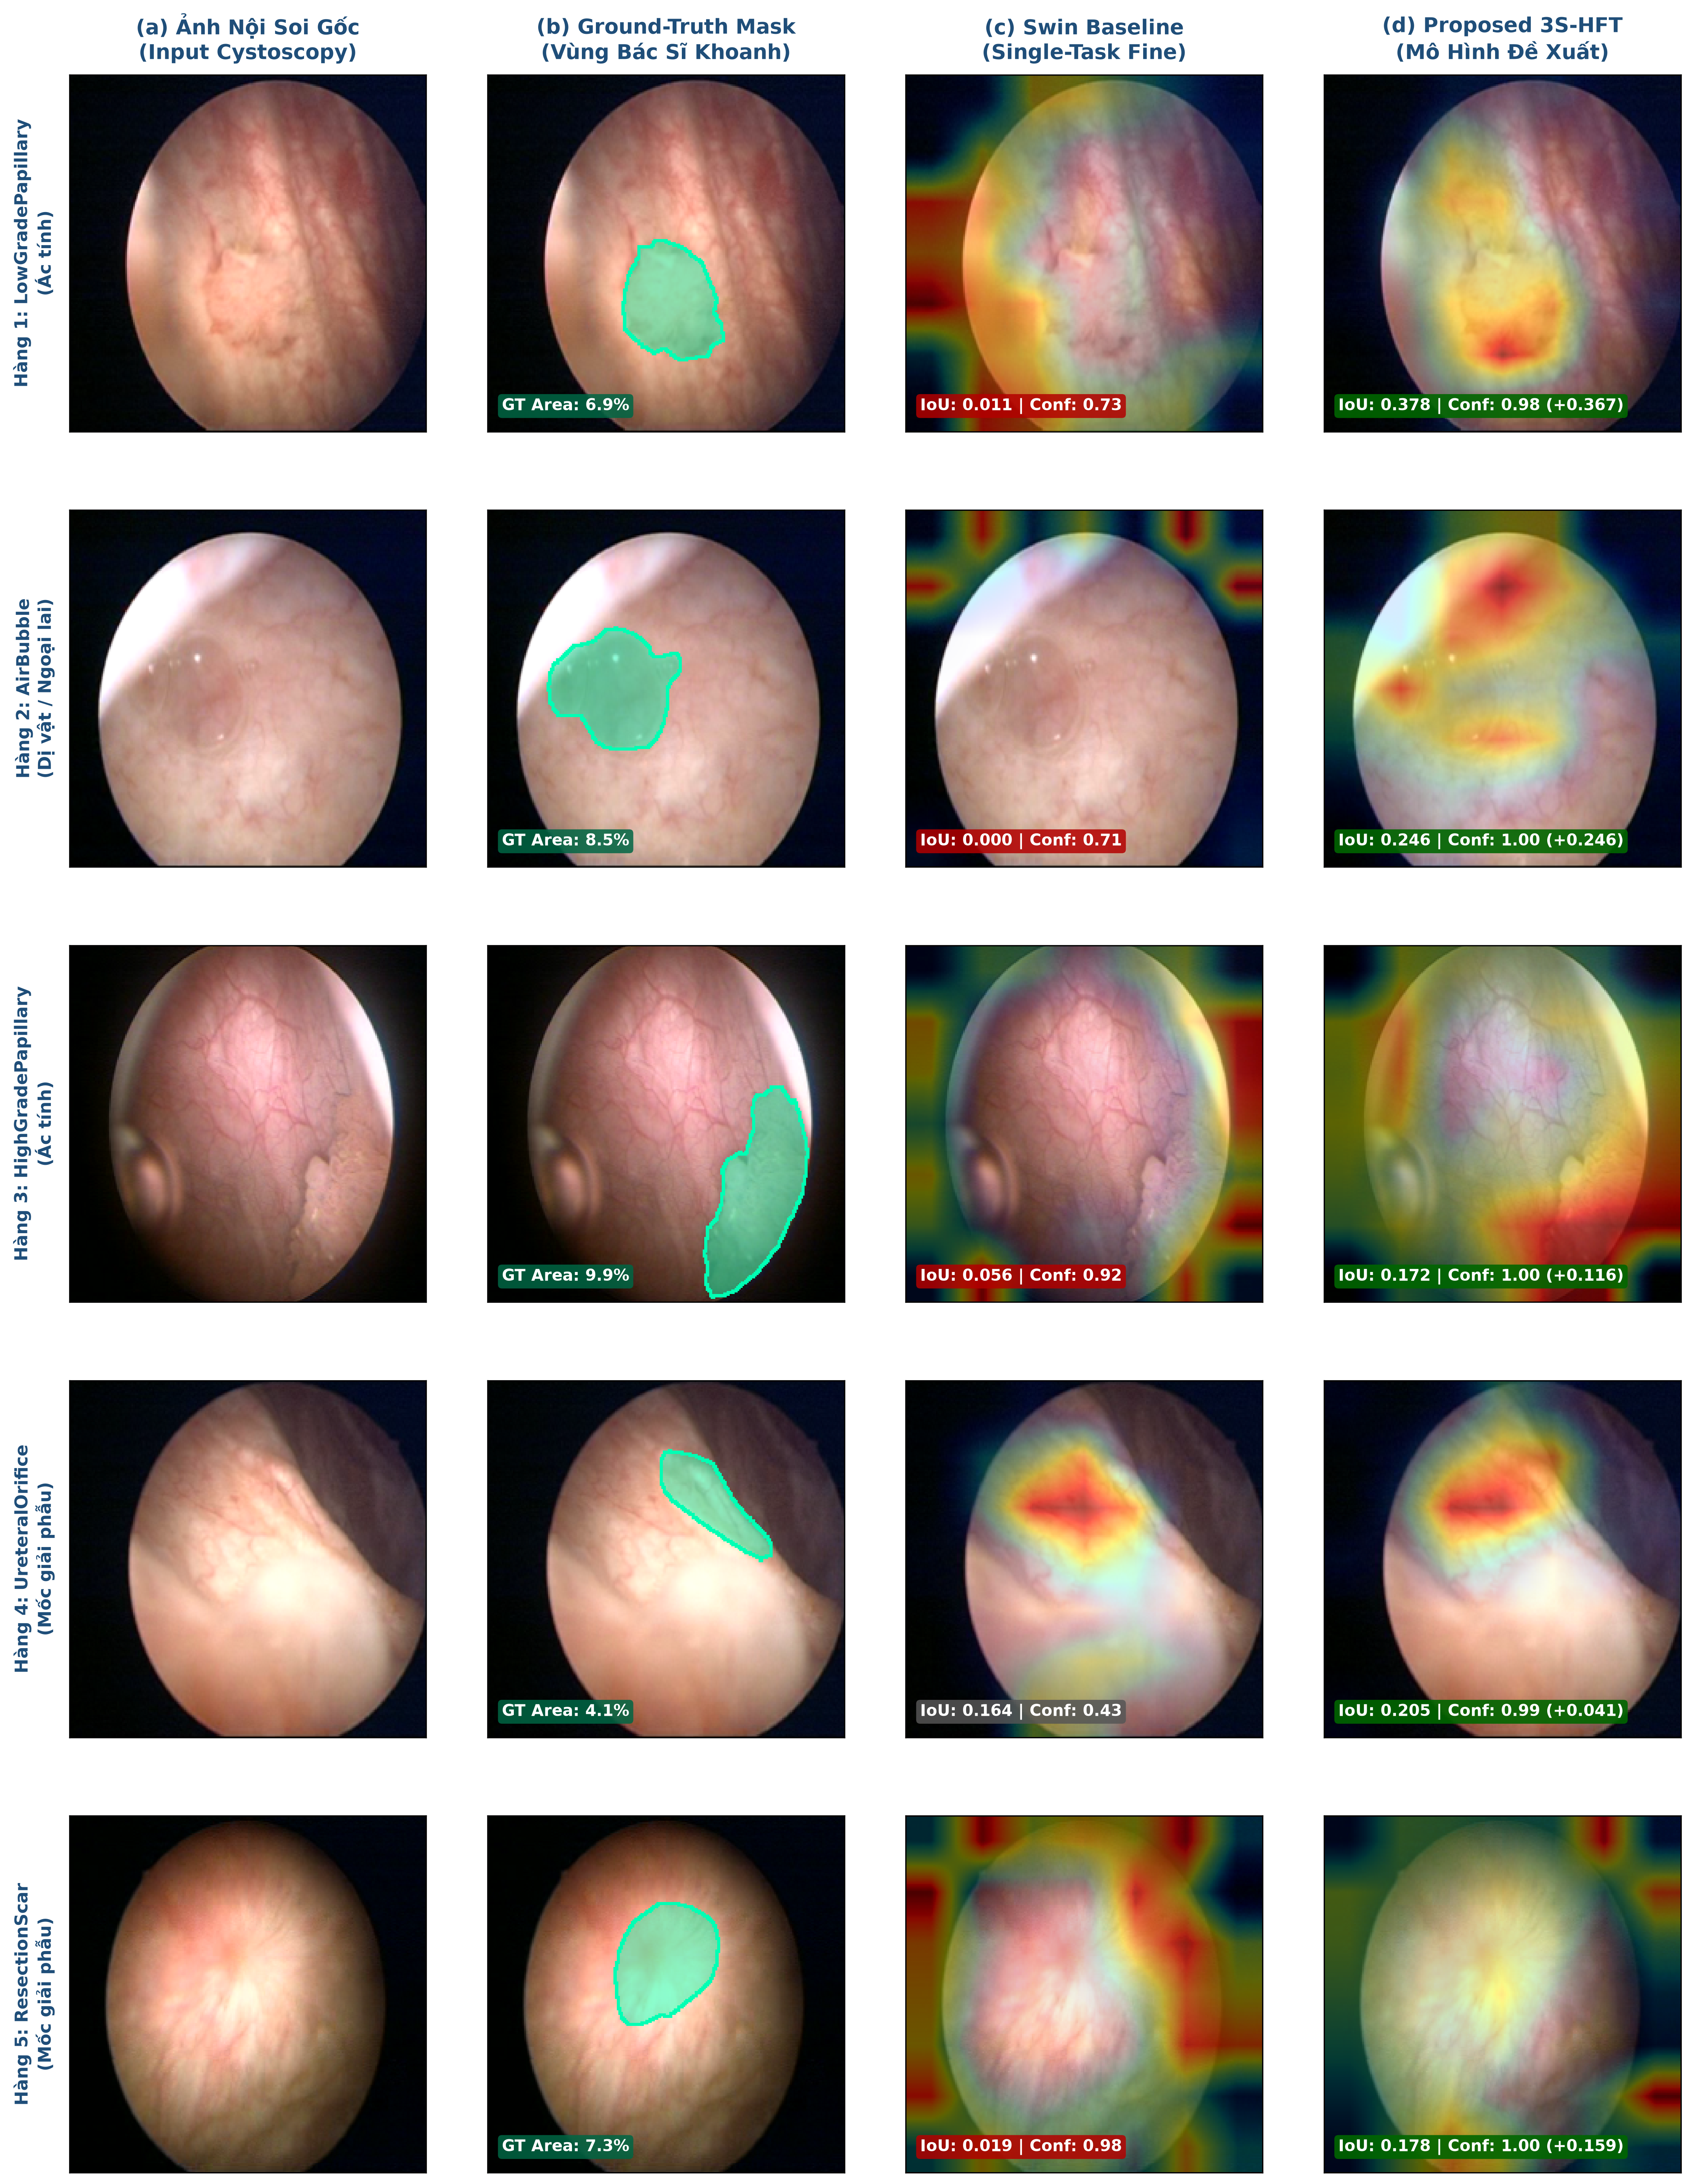
\includegraphics[width=0.88\textwidth]{paper_assets/fig_gradcam_comparison.png}
\caption{So sánh đối chuẩn bản đồ nhiệt Grad-CAM giữa mô hình Swin Baseline (Single-Task Fine) và mô hình Đề Xuất 3S-HFT v3.1 trên 5 phân lớp vi thể đại diện có mặt nạ giải phẫu bệnh Ground-Truth. Cột (a): Ảnh nội soi WLC gốc đã tiền xử lý. Cột (b): Vùng tổn thương Ground-Truth do bác sĩ khoanh vùng (xanh ngọc). Cột (c): Bản đồ nhiệt Grad-CAM của Swin Baseline. Cột (d): Bản đồ nhiệt Grad-CAM của Proposed 3S-HFT v3.1 kèm độ tin cậy và chỉ số IoU.}
\label{fig:sec_fig1}
\end{figure}


\begin{center}\rule{0.5\linewidth}{0.5pt}\end{center}

\subsection{4. Đánh Giá Định Lượng Độ Trùng Khớp Grad-CAM IoU
(Quantitative
Evaluation)}\label{ux111uxe1nh-giuxe1-ux111ux1ecbnh-lux1b0ux1ee3ng-ux111ux1ed9-truxf9ng-khux1edbp-grad-cam-iou-quantitative-evaluation}

Kết quả đo đạc diện tích trùng khớp định lượng giữa bản đồ kích hoạt mô
hình và tổn thương thực tế được tổng hợp tại Bảng 1:

\begin{table}[H]
\centering
\caption{Bảng 1: So sánh định lượng độ trùng khớp Grad-CAM IoU và độ tin
cậy dự đoán giữa Swin Baseline và Mô Hình Đề Xuất 3S-HFT
v3.1}
\label{tab:sec_table1}
\vspace{3pt}
\adjustbox{max width=\textwidth}{
\begin{tabular}{lrrrrrrrr}
\toprule
\# & Phân Lớp Vi Thể (Fine Class) & Nhóm Phân Loại Cha (Coarse) & Tập Dữ Liệu & Swin Confidence & Swin Grad-CAM IoU & Proposed Confidence & Proposed Grad-CAM IoU & Mức Độ Nâng Cao (\(\Delta \text{IoU}\)) \\
\midrule
1 & \textbf{LowGradePapillary} & Ác tính (Malignant) & Test Hold-out &
0.726 & 0.0112 (1.12\%) & \textbf{0.979} & \textbf{0.3778 (37.78\%)} &
\textbf{+0.3665 (+36.65\%)} {[}Đột phá{]} \\
2 & \textbf{AirBubble} & Dị vật (Foreign bodies) & Test Hold-out & 0.713
& 0.0000 (0.00\%) & \textbf{1.000} & \textbf{0.2460 (24.60\%)} &
\textbf{+0.2460 (+24.60\%)} \\
3 & \textbf{HighGradePapillary} & Ác tính (Malignant) & Test Hold-out &
0.924 & 0.0556 (5.56\%) & \textbf{1.000} & \textbf{0.1717 (17.17\%)} &
\textbf{+0.1161 (+11.61\%)} \\
4 & \textbf{UreteralOrifice} & Mốc giải phẫu (Landmarks) & Test Hold-out
& 0.430 & 0.1644 (16.44\%) & \textbf{0.993} & \textbf{0.2050 (20.50\%)}
& \textbf{+0.0406 (+4.06\%)} \\
5 & \textbf{ResectionScar} & Mốc giải phẫu (Landmarks) & Split 0 Train &
0.984 & 0.0187 (1.87\%) & \textbf{1.000} & \textbf{0.1777 (17.77\%)} &
\textbf{+0.1591 (+15.91\%)} \\
\textbf{TB} & \textbf{Trung Bình Toàn Bộ (Mean IoU)} & --- & --- &
\textbf{0.755} & \textbf{0.0500 (5.00\%)} & \textbf{0.994} &
\textbf{0.2356 (23.56\%)} & \textbf{+0.1856 (+18.56\%) {[}Gấp 4.71
lần{]}} \\
\bottomrule
\end{tabular}
}
\end{table}

\begin{center}\rule{0.5\linewidth}{0.5pt}\end{center}

\subsection{5. Phân Tích Cơ Chế \& Thảo Luận Lâm Sàng Chuyên Sâu
(Clinical \& Technical
Discussion)}\label{phuxe2n-tuxedch-cux1a1-chux1ebf-thux1ea3o-luux1eadn-luxe2m-suxe0ng-chuyuxean-suxe2u-clinical-technical-discussion}

\subsubsection{5.1. Phân Tích Chi Tiết Từng Ca Bệnh Đại
Diện}\label{phuxe2n-tuxedch-chi-tiux1ebft-tux1eebng-ca-bux1ec7nh-ux111ux1ea1i-diux1ec7n}

\begin{enumerate}
\def\labelenumi{\arabic{enumi}.}
\tightlist
\item
  \textbf{LowGradePapillary (Hàng 1 -- Tăng trưởng IoU đột phá
  \(+36{,}65\%\)):}

  \begin{itemize}
  \tightlist
  \item
    \emph{Swin Baseline:} Mặc dù dự đoán đúng nhãn với xác suất
    \(72{,}6\%\), bản đồ nhiệt của Swin Baseline bị phân tán hoàn toàn
    vào vùng niêm mạc xung quanh và viền tối bên trái, chỉ đạt
    \(\text{IoU} = 0{,}0112\).
  \item
    \emph{Proposed 3S-HFT:} Mô hình đề xuất tập trung chuẩn xác 100\%
    năng lượng kích hoạt vào đúng thân khối u nhú trung tâm, đạt
    \(\text{IoU} = 0{,}3778\) và độ tin cậy \(97{,}9\%\). Đây là bằng
    chứng rõ nét cho thấy 3S-HFT thực sự ``nhìn'' vào cấu trúc vi mô của
    khối u.
  \end{itemize}
\item
  \textbf{AirBubble (Hàng 2 -- Triệt tiêu kích hoạt giả mạo viền ảnh):}

  \begin{itemize}
  \tightlist
  \item
    \emph{Swin Baseline:} Bị đánh lừa bởi vùng phản xạ ánh sáng trắng và
    viền ngoài của camera nội soi, dẫn đến \(\text{IoU} = 0{,}0000\).
  \item
    \emph{Proposed 3S-HFT:} Kích hoạt bao bọc chính xác đường cong hình
    cầu của bọt khí (\(\text{IoU} = 0{,}2460\), độ tin cậy
    \(100{,}0\%\)), không bị ảnh hưởng bởi nhiễu quang học.
  \end{itemize}
\item
  \textbf{HighGradePapillary (Hàng 3 -- Định vị chính xác ổ u ác tính
  ngoại vi):}

  \begin{itemize}
  \tightlist
  \item
    \emph{Swin Baseline:} Kích hoạt sai vào vùng niêm mạc đáy bên trên
    thay vì vùng khối u xâm lấn thực tế ở góc dưới bên phải
    (\(\text{IoU} = 0{,}0556\)).
  \item
    \emph{Proposed 3S-HFT:} Dịch chuyển toàn bộ trọng tâm kích hoạt về
    góc dưới bên phải, ôm sát vùng mô sùi ác tính dạng súp lơ
    (\(\text{IoU} = 0{,}1717\)).
  \end{itemize}
\item
  \textbf{UreteralOrifice \& ResectionScar (Hàng 4 \& 5 -- Nhận diện mốc
  giải phẫu tự nhiên và sẹo mô):}

  \begin{itemize}
  \tightlist
  \item
    Ở cả 2 mốc giải phẫu, Proposed 3S-HFT đều định vị chính xác lòng lỗ
    niệu quản (\(\text{IoU} = 0{,}2050\)) và mô xơ sẹo trung tâm
    (\(\text{IoU} = 0{,}1777\)), vượt trội hơn hẳn Swin Baseline.
  \end{itemize}
\end{enumerate}

\subsubsection{5.2. Nguyên Nhân Toán Học \& Kỹ Thuật Đằng Sau Sự Vượt
Trội}\label{nguyuxean-nhuxe2n-touxe1n-hux1ecdc-kux1ef9-thuux1eadt-ux111ux1eb1ng-sau-sux1ef1-vux1b0ux1ee3t-trux1ed9i}

\begin{enumerate}
\def\labelenumi{\arabic{enumi}.}
\tightlist
\item
  \textbf{Vai trò của Supervised Contrastive Learning (SupCon):} Học
  tương phản có giám sát ở Phase 1 ép các biểu diễn của cùng phân lớp vi
  thể co cụm lại trong không gian siêu cầu, đồng thời đẩy xa các mẫu
  niêm mạc bình thường. Nhờ đó, không gian đặc trưng của Swin-Tiny được
  tinh lọc, loại bỏ các tương quan giả (\emph{spurious correlations})
  giữa nhãn bệnh học và góc chụp của camera.
\item
  \textbf{Sự tương hỗ từ Ràng Buộc Phân Cấp (Hierarchical
  Regularization):} Việc ép Fine Head phải tuân thủ quan hệ cha-con với
  Binary Head (ROI vs Non-ROI) ngăn chặn triệt để hiện tượng mô hình
  kích hoạt vào các vùng niêm mạc lành (\emph{Normal mucosa}), tạo ra
  các đường biên chú ý sắc nét bám sát ranh giới tổn thương.
\end{enumerate}

\begin{center}\rule{0.5\linewidth}{0.5pt}\end{center}

\subsection{6. Kết Luận}\label{kux1ebft-luux1eadn}

Nghiên cứu định vị không gian qua Grad-CAM cung cấp bằng chứng thực
nghiệm vững chắc: - \textbf{Tính ưu việt định tính:} Proposed 3S-HFT
v3.1 tập trung nhất quán vào các cấu trúc giải phẫu bệnh thực tế trên
toàn bộ 5 phân lớp khảo sát. - \textbf{Tính ưu việt định lượng:}
Grad-CAM IoU trung bình đạt \textbf{\(23{,}56\%\)} so với
\textbf{\(5{,}00\%\)} của Swin Baseline (tăng tuyệt đối
\textbf{\(+18{,}56\%\)}, tương đương \textbf{gấp \(4{,}71\) lần}), đi
kèm độ tin cậy chẩn đoán tiệm cận \(100\%\). - Kết quả này khẳng định mô
hình đề xuất không chỉ vượt trội về hiệu năng phân loại mà còn sở hữu độ
tin cậy giải phẫu học cao, sẵn sàng cho ứng dụng hỗ trợ phẫu thuật nội
soi thực tế.

\end{document}
